\documentclass{article}
%\usepackage[OT4]{fontenc}
%\usepackage[polish]{babel}
\usepackage{polski}
\usepackage[utf8]{inputenc}
\usepackage{apacite}
\usepackage{natbib}
\usepackage{caption}
\usepackage{booktabs}
\usepackage{colortbl, xcolor}
\usepackage{tabularx}
\usepackage{graphicx}
\usepackage{multirow}
\usepackage{epstopdf}

\author{Michał Burdukiewicz, Przemysław Gagat}
\title{Moduł bioinformatyczny bazy metanogenów\linebreak \vskip{} 
\large{Projekt badawczy Doktoranckiego Koła Naukowego Bioinformatyki}} 
\date{}

\AtBeginDocument{%
  \renewcommand{\tablename}{Tab.}
} 

\AtBeginDocument{%
  \renewcommand{\figurename}{Rys.}
} 

\begin{document}

\maketitle

\section{Założenia i cel projektu badawczego}

Metanogeny to grupa archebakterii, które w procesie oddychania produkują metan. 
Ze względu na istotną rolę w różnych środowiskach beztlenowych, takich jak 
przewód pokarmowy czy gleba, metanogeny są obiecującym obiektem badań 
naukowych, zarówno pod względem zastosowań przemysłowych jak i analiz 
filogenetycznych.

Baza Methanogens~\citep{jablonski_methanogenic_2015} 
(\url{http://metanogen.biotech.uni.wroc.pl/}) jest największym 
istniejącym zbiorem danych dotyczących warunków hodowlanych metanogenów. Nie 
zawiera jednak dodatkowych informacji, które umożliwiłyby przeprowadzenie 
analiz filogenetycznych.

Zadaniem badawczym jest dodanie do bazy Methanogens zestawu narzędzi 
umożliwiających bioinformatyczną analizę metanogenów. Wymaga to zarówno 
stworzenia narzędzi dostępnych jako web servers, a także uzupełnienia bazy o 
dane istotne z punktu widzenia biologii obliczeniowej. Dodatkowo, ponieważ 
obecne narzędzia wizualizacyjne bazy są w tej chwili dość ograniczone, zostaną 
poszerzone w 
trakcie trwania projektu.


\section{Obecny stan badań}

Trzonem informacji zgromadzonych w bazie Methanogens są wyczerpujące dane na 
temat warunków hodowlanych metanogenów. Informacje te zostały pozyskane ręcznie 
z różnych źródeł i wystandaryzowane. Dodatkową zaletą bazy Methanogens są 
narzędzia wizualizacyjne pozwalające na interaktywne porównywanie ze sobą 
różnych metanogenów pod względem ich cech fenotypowych. 

Jakkolwiek istniejące funkcje wizualizacyjne są bardzo pomocne, to obecnie brak 
narzędzi umożliwiających jednoczesną wizualizację więcej niż dwóch zmiennych. 
To ograniczenie wydaje się szczególnie dotkliwe biorąc pod uwagę 
wielowymiarowość danych zgromadzonych w bazie Methanogenes. 

Istotnym brakiem bazy Methanogenes jest nieobecność w niej sekwencji 
nukleinowych i aminokwasowych metanogenów. Taka informacja jest cenna we 
wszelkiego rodzaju metodach biologii obliczeniowej, w tym 
badaniach filogenetycznych. Wzbogacenie bazy metanogenów o odpowiednie 
sekwencje nukleinowe i aminokwasowe z pewnością uczyni ją przydatniejszą dla 
szerszego grona użytkowników pod warunkiem dodania do bazy oprogramowania 
umożliwiające efektywne przeszukiwanie zbioru sekwencji.

\section{Metody}

\begin{figure}[ht]
\centering
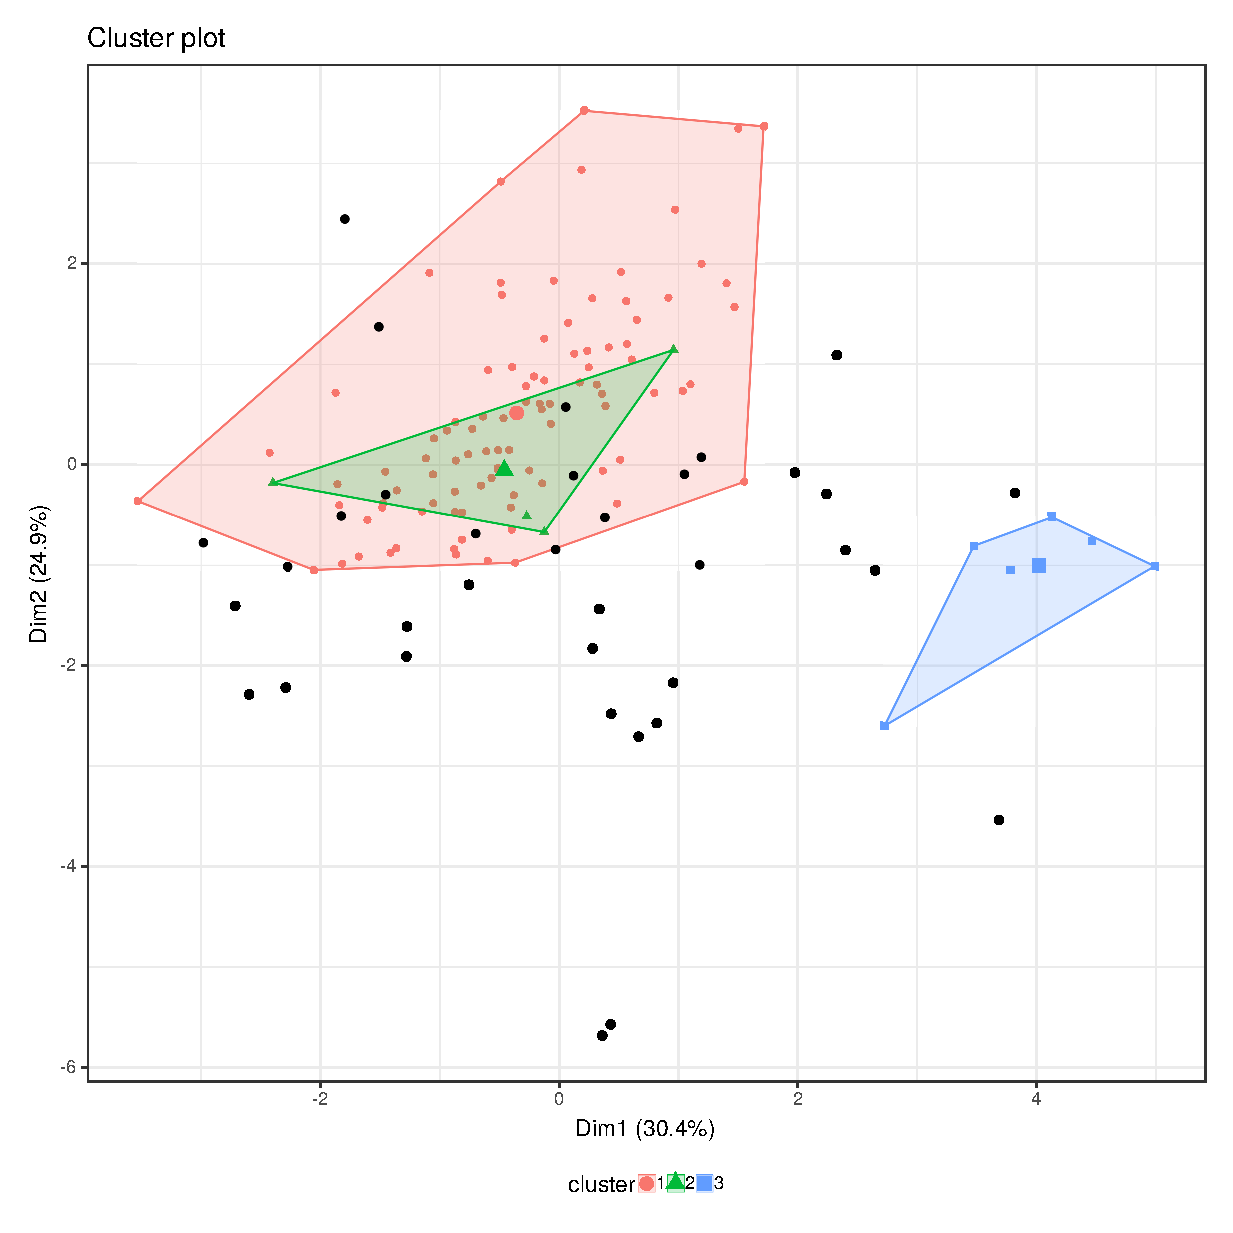
\includegraphics[width=0.75\textwidth]{cluster.eps}
\caption{Przykładowa analiza skupień danych zebranych w bazie Methanogens.}
\label{fig:cluster}
\end{figure}

\subsection{Pozyskanie i przeszukiwanie sekwencji metanogenów}

Sekwencje nukleotydowe i aminokwasowe metanogenów zostaną pozyskane z baz NCBI, 
odpowiednio Nucletide i Protein. W celu automatyzacji procesu, sekwencje zostaną 
pozyskane z użyciem EUtils API udostępnionym przez NCBI 
(\url{http://www.ncbi.nlm.nih.gov/books/NBK25500/}).

W celu zagwarantowanie większej jakości pozyskanych rekordów, sekwencje zostaną 
poddane ręcznej kuracji. 

Zgromadzony zbiór sekwencji będzie można przeszukiwać dzięki lokalnej instancji 
algorytmu Blast \citep{altschul_basic_1990}, który zostanie udostępniony 
użytkownikom bazy.

\subsection{Analiza częstościowa}

Baza zostanie uzupełniona o dodatkowy moduł, web server odpowiedzialny za 
wizualizację sekwencji za pomocą analizy częstościowej. Typowa analiza 
występowania pojedynczych reszt nukletydowych lub aminokwasowych zostanie 
rozszerzona o analizę n-gramów, ciągłych lub nieciągłych podsekwencji długości 
$n$. Obliczenia zostaną wykonane dzięki narzędziom z pakietu \textit{biogram} 
\citep{burdukiewicz_biogram:_2017}, a web server zostanie zrealizowany w 
technologii \textit{shiny}.

\subsection{Analiza skupień}

Web server dedykowany analizie skupień danych zgromadzonych w bazie zostanie 
oparty o algorytm klasteryzacji gęstościowej \citep{ester_density-based_1996}. 
Metodę 
tę wybraną ze względu na odporność na zaszumienie danych i szybkość działania. 
Analiza będzie w pełni interaktywna, co oznacza, że użytkownik będzie mógł 
wybrać interesujące go cechy, a następnie określić parametry działania 
algorytmu. Wynikiem analizy nie będą tylko dane liczbowe, ale również graficzna 
reprezentacja znalezionych klastrów \ref{fig:cluster}.



\section{Czas realizacji projektu}

Projekt będzie realizowany w okresie 1.06.2017 do 30.11.2017.

\section{Planowane wydatki}

Łączny koszt projektu badawczego to 9 560,00 zł. Ze względu na możliwość zmiany 
cen poszczególnych produktów, Doktoranckie Koło Naukowe Bioinformatyki zwraca 
się o przyznanie 10 000,00 zł.

\begin{table}[!htbp]
\centering
\caption{Kosztorys projektu badawczego.}
\begin{tabular}{rrr}
\cline{1-2}
\multicolumn{1}{|c}{Nazwa}                                   & \multicolumn{1}{|c|}{Koszt}   &  \\ \cline{1-2}
\multicolumn{1}{|c}{Akcesoria niezbędne w realizacji zadań badawczych}   & 
\multicolumn{1}{|c|}{5560,00 zł} &  \\ \cline{1-2}
\multicolumn{1}{|c}{Wyjazdy konferencyjne}   & 
\multicolumn{1}{|c|}{4 000,00 zł} &  \\ \cline{1-2}
Łącznie    & 9 560,00 zł                    & 
\end{tabular}
\end{table}

\subsection{Akcesoria niezbędne w realizacji zadań badawczych}

Właściwe zrealizowanie projektu badawczego wymaga dokupienie akcesoriów i 
sprzętu komputerowego (Tab.~\ref{tab:akcesoria}), takich jak klawiatury i 
monitor niezbędne do wykorzystania stanowisk komputerowych udostępnionych przez 
Zakład Genomiki. Konieczna jest również rozbudowa tych stanowisk poprzez 
dokupienie pamięci DDR. Wykonanie części zadań badawczych nie byłaby możliwa 
gdyby nie komputery przenośne udostępnione członkom Koła przez Zakład Genomiki. 
Bezpieczny transport otrzymanego sprzętu wymaga zakupu specjalnych plecaków na 
laptopy.

\begin{table}[]
\centering
\caption{Koszty akcesoriów niezbędnych w realizacji zadań badawczych.}
\label{tab:akcesoria}
\begin{tabular}{cccc}
\hline
\multicolumn{1}{|c|}{Nazwa}             & \multicolumn{1}{c|}{Koszt jednostkowy} 
& \multicolumn{1}{c|}{Liczba sztuk} & \multicolumn{1}{c|}{Łączny koszt} \\ 
\hline
\multicolumn{1}{|c|}{pamięć DDR3 8GB}   & \multicolumn{1}{c|}{250}               
& \multicolumn{1}{c|}{12}           & \multicolumn{1}{c|}{3000,00 zł}   \\ 
\hline
\multicolumn{1}{|c|}{Monitor 27’}       & \multicolumn{1}{c|}{1000}              
& \multicolumn{1}{c|}{1}            & \multicolumn{1}{c|}{1000,00 zł}   \\ 
\hline
\multicolumn{1}{|c|}{kabel DVI-D 1m}    & \multicolumn{1}{c|}{200}               
& \multicolumn{1}{c|}{1}            & \multicolumn{1}{c|}{200,00 zł}    \\ 
\hline
\multicolumn{1}{|c|}{kabel HDMI 5m}     & \multicolumn{1}{c|}{160}               
& \multicolumn{1}{c|}{1}            & \multicolumn{1}{c|}{160,00 zł}    \\ 
\hline
\multicolumn{1}{|c|}{klawiatura USB}    & \multicolumn{1}{c|}{400}               
& \multicolumn{1}{c|}{2}            & \multicolumn{1}{c|}{800,00 zł}    \\ 
\hline
\multicolumn{1}{|c|}{torba na laptopa}  & \multicolumn{1}{c|}{200}               
& \multicolumn{1}{c|}{1}            & \multicolumn{1}{c|}{200,00 zł}    \\ 
\hline
\multicolumn{1}{|c|}{plecak na laptopa} & \multicolumn{1}{c|}{200}               
& \multicolumn{1}{c|}{1}            & \multicolumn{1}{c|}{200,00 zł}    \\ 
\hline
\multicolumn{1}{l}{}                    & \multicolumn{1}{l}{}                   
& \multicolumn{1}{l}{}              & \multicolumn{1}{l}{5 560,00 zł}   
\end{tabular}
\end{table}

\subsection{Wyjazdy konferencyjne}

Utworzone web servery zostaną zaprezentowane podczas konferencji International 
Society for Computational Biology w Pradze (21-26.07.2017). Dofinansowane 
zostaną dwa wyjazdy na konferencję.

\begin{table}[!htbp]
\centering
\caption{Kosztorys wyjazdów konferencyjnych.}
\begin{tabular}{lllll}
\cline{1-4}
\multicolumn{1}{|c|}{Nazwa}                     & \multicolumn{1}{c|}{Cena (szt.)} & \multicolumn{1}{c|}{Liczba} & \multicolumn{1}{c|}{Łączna cena} &  \\ \cline{1-4}
\multicolumn{1}{|c|}{Dofinansowanie wyjazdu} & \multicolumn{1}{c|}{2 000 zł}    
 & \multicolumn{1}{c|}{2}      & \multicolumn{1}{c|}{4 000 zł}     &  \\ 
\cline{1-4}
                                                &                                
  & Łącznie:                    & 4 000,00 zł                          & 
\end{tabular}
\end{table}


\bibliographystyle{apacite} 
\bibliography{methanogens}

\end{document}